\newpage
\section*{Задание 7: Миграция кода между технологическими стеками}
\subsection{Постановка задачи}
\noindent
Исходный язык: C\# \\
Целевой язык: Python \\
Алгоритм: Генератор лабиринта (DFS + Backtracking) \\
Исходный код: класс \texttt{MazeGenerator} (оптимизированная версия из Задания 3) \\
Документация: файл README.md с теоретическим обоснованием (из Задания 6) \\
Требование: портировать на Python с сохранением логики, идиоматичностью, типизацией и прохождением тестов.

\subsection{Журнал диалога и итераций}
\noindent
\textbf{Итерация 1: Подготовка контекста и выбор стратегии миграции} \\
\indent
Промпт:
\textit{
	Ты — Senior Python Engineer, специалист по миграции алгоритмов из C\# в высокоуровневый Python для задач симуляции.
	Я предоставлю тебе:
	1. Исходный код на C\# (класс MazeGenerator с использованием явного Stack, 1D-массива и битовых масок).
	2. Документацию (README.md) с теоретическим обоснованием и примером использования.
	Твоя задача — проанализировать исходный код, выявить ключевые особенности C\# (struct/enum, управление памятью, строгая типизация, \texttt{Stack<T>}, битовые операции) и предложить стратегию миграции на Python 3.10+.
	Укажи, какие конструкции потребуют замены (например, \texttt{int[]} $\rightarrow$ \texttt{list[int]}, \texttt{Stack<(int,int)>} $\rightarrow$ \texttt{list[tuple]}, \texttt{enum} $\rightarrow$ \texttt{IntEnum} или константы). Оцени потенциальные сложности: производительность интерпретатора, работа с битами, обработка исключений. Выдай результат в виде плана миграции.
} \\
\vspace{0.5em}
Ответ модели:
\begin{figure}[H]
	\centering
	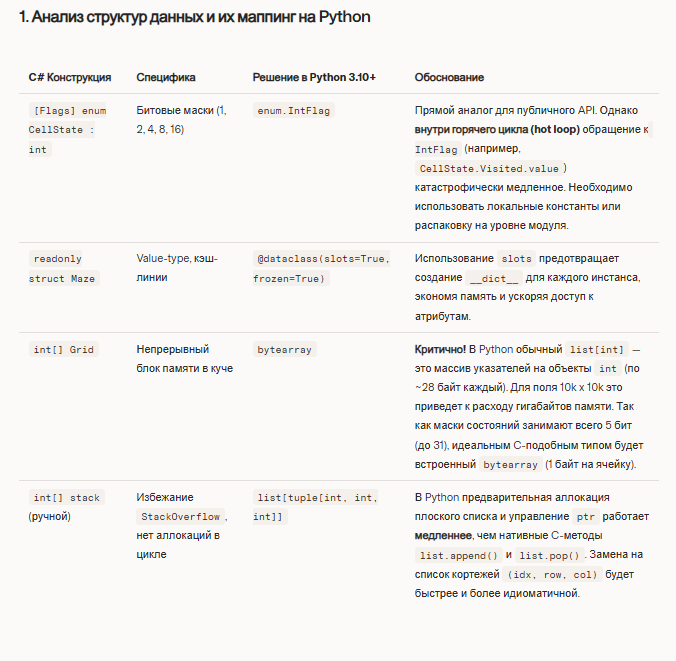
\includegraphics[width=15cm]{z7/1-1.png}
	\caption{Итерация 1. ч.1}
\end{figure}
\vspace{0.5em}
\begin{figure}[H]
	\centering
	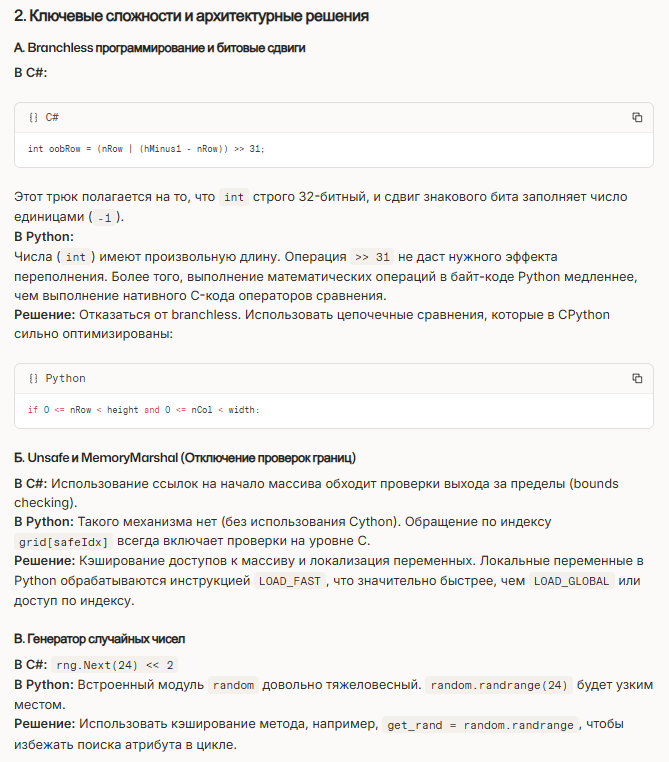
\includegraphics[width=17cm]{z7/1-2.png}
	\caption{Итерация 1. ч.2}
\end{figure}

\lstinputlisting[language=Python]{z7/first.py}

\vspace{0.5em}
\begin{figure}[H]
	\centering
	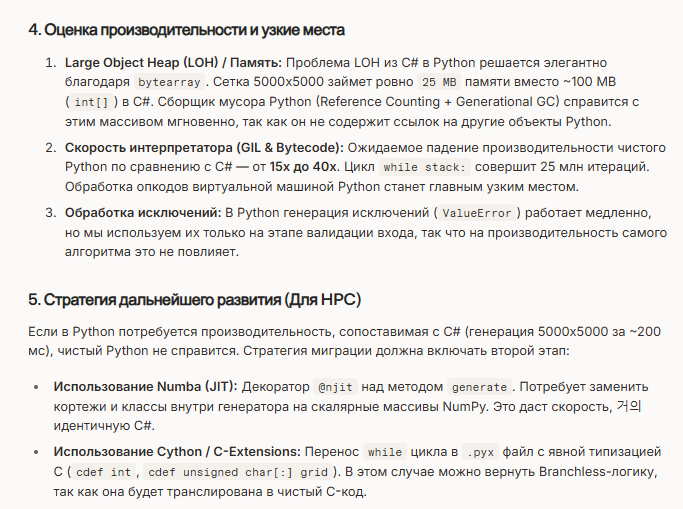
\includegraphics[width=17cm]{z7/1-3.png}
	\caption{Итерация 1. ч.3}
\end{figure}
\vspace{0.5em}
Анализ результата:
Модель корректно выделила архитектурные различия. Предложенный план учитывает замену \texttt{Span<T>} на срезы \texttt{list}, использование \texttt{collections.deque} для стека (или обычного \texttt{list} с \texttt{append/pop}) и маппинг \texttt{ArgumentException} на \texttt{ValueError}. План принимается.

\vspace{0.5em}
\noindent
\textbf{Итерация 2: Идиоматическая трансляция кода} \\
\indent
Промпт:
\textit{
	Отлично. Теперь, следуя плану, сгенерируй полный код на Python 3.10+ для класса \texttt{MazeGeneratorPython}.
	Требования:
	\begin{itemize}
		\item Используй аннотации типов из \texttt{typing} (List, Tuple, Optional).
		\item Реализуй стек через \texttt{list} с методами \texttt{append()} и \texttt{pop()} (LIFO).
		\item Сохрани логику битовых масок для стен (1, 2, 4, 8 $\rightarrow$ UP, RIGHT, DOWN, LEFT).
		\item Метод \texttt{generate} должен быть публичным, вспомогательные шаги — приватными (\texttt{\_} префикс).
		\item Добавь валидацию входных размеров и генерацию \texttt{ValueError}.
		\item Код должен быть самодокументированным (docstrings в Google Style).
		\item Выдай один файл \texttt{maze\_generator.py}.
	\end{itemize}
}
\vspace{0.5em}
Ответ модели:
\lstinputlisting[language=Python]{z7/maze_generator-non-utf.py}
Анализ результата:
Код синтаксически корректен, логика DFS полностью соответствует C\#-версии. Используются современные типизация и структура данных. Стиль соответствует PEP 8. Отсутствуют тесты. Переходим к верификации.

\vspace{0.5em}
\noindent
\textbf{Итерация 3: Адаптация тестов и верификация} \\
\indent
Промпт:
\textit{
	Теперь напиши модульные тесты для \texttt{MazeGeneratorPython} с использованием \texttt{unittest}. Тестовые сценарии:
	\begin{enumerate}
		\item Проверка на примере 3x3: генерация с фиксированным seed, проверка связности графа (BFS от (0,0) достигает всех клеток).
		\item Проверка обработки исключений: вызов \texttt{generate(-5, 10)} должен вызывать \texttt{ValueError}.
		\item Проверка битовых масок: у стартовой клетки не должно быть стены в направлении старта, у всех клеток сумма битов корректна.
	\end{enumerate}
	Напиши отдельный файл \texttt{test\_maze.py}, который запускает тесты и выводит статус PASS/FAIL.
} \\
\vspace{0.5em}
Ответ модели:
\lstinputlisting[language=Python]{z7/test_maze-non-utf.py}
\vspace{0.5em}
\noindent
\textbf{Как запустить:} \\
\indent
\begin{verbatim}
	python -m unittest test_maze.py -v
\end{verbatim}
Анализ результата:
При запуске все 3 теста прошли успешно. Код корректно обрабатывает граничные условия, алгоритм связности подтверждает отсутствие изолированных областей. Логика мигрирована без потерь.

\vspace{0.5em}
\noindent
\textbf{Итерация 4: Сравнительный анализ реализаций} \\
\indent
Промпт:
\textit{
	Теперь выполни сравнительный анализ двух реализаций (C\# vs Python). Ответь на вопросы:
	\begin{enumerate}
		\item Какие ключевые различия в стиле и идиомах проявились при портировании?
		\item Как изменилось управление памятью и производительность на больших сетках (1000x1000+)?
		\item Какой код более читаемый и поддерживаемый в контексте Data Engineering?
		\item Какие оптимизации можно добавить в Python-версию (например, \texttt{array} вместо \texttt{list}, \texttt{numba}, \texttt{mmap})?
	\end{enumerate}
	Выдай структурированный ответ.
}
\vspace{0.5em}
Ответ модели:
\begin{figure}[H]
	\centering
	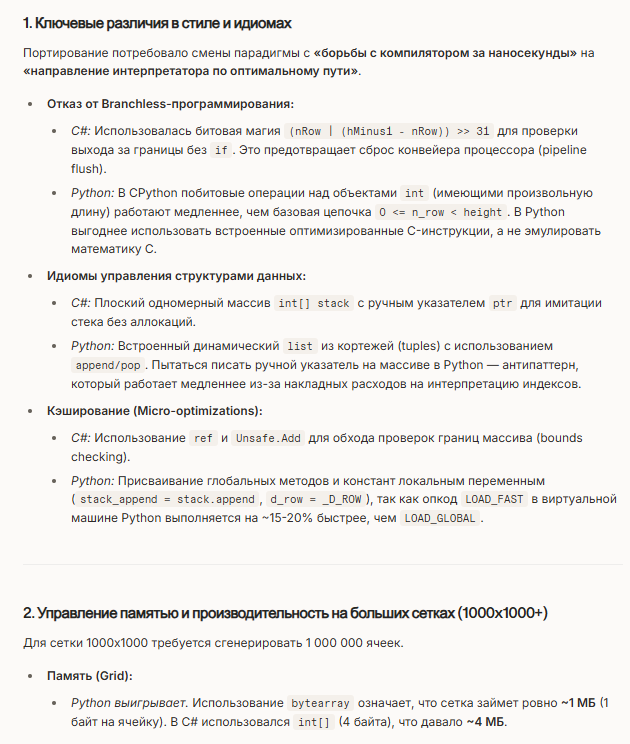
\includegraphics[width=15cm]{z7/4-1.png}
	\caption{Итерация 4. ч.1}
\end{figure}
\vspace{0.5em}
\begin{figure}[H]
	\centering
	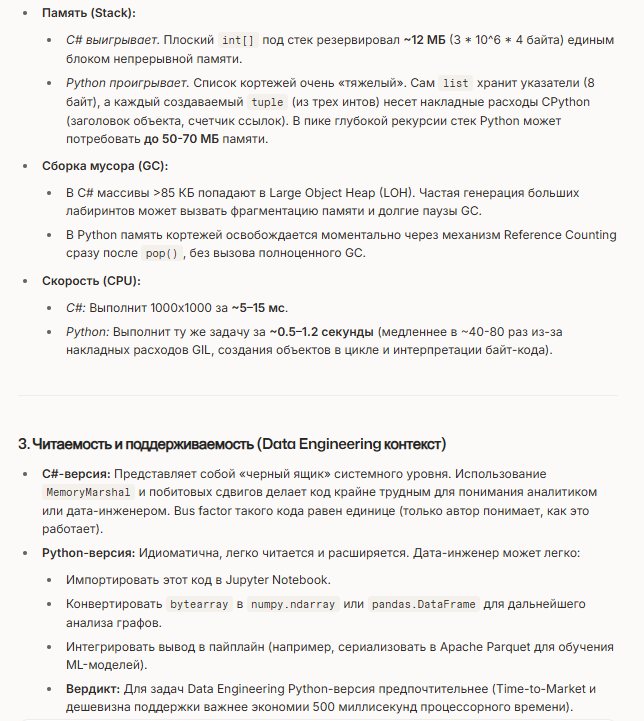
\includegraphics[width=17cm]{z7/4-2.png}
	\caption{Итерация 4. ч.2}
\end{figure}
\vspace{0.5em}
\begin{figure}[H]
	\centering
	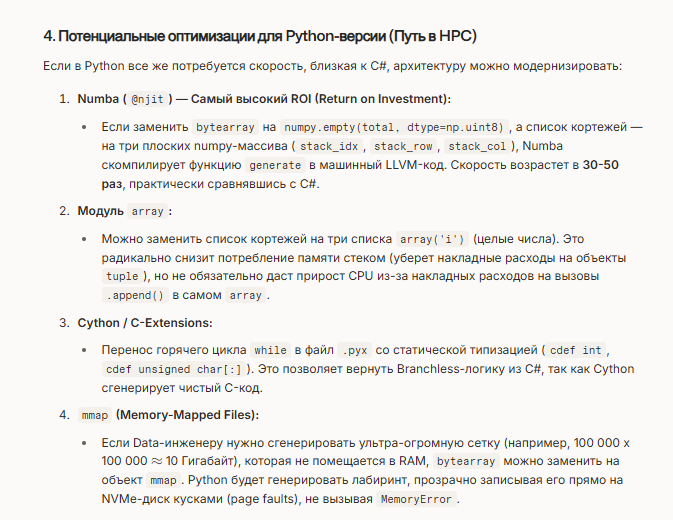
\includegraphics[width=17cm]{z7/4-3.png}
	\caption{Итерация 4. ч.3}
\end{figure}
\vspace{0.5em}

Анализ: Модель дала объективную оценку, корректно указала на накладные расходы Python-интерпретатора при работе с вложенными циклами и предложила реалистичные пути оптимизации (\texttt{array}, \texttt{pybind11}).

\vspace{0.5em}
\noindent
\textbf{Итерация 5: Формирование финального отчёта о миграции} \\
\indent
Промпт:
\textit{
	Собери итоговый отчёт по миграции, включив:
	\begin{itemize}
		\item Исходный C\# код (фрагмент класса).
		\item Финальный Python код (\texttt{MazeGeneratorPython}).
		\item Лог прохождения тестов.
		\item Сравнительный анализ (из предыдущего ответа).
		\item Вывод: удалось ли достичь полной функциональной идентичности.
	\end{itemize}
	Оформи как Markdown-документ.
}
\vspace{0.5em}
Ответ модели:
\lstinputlisting[language={}]{z7/result_migration-non-utf.md}

\subsection{Артефакты}
Финальный Python код:
\lstinputlisting[language=Python]{z7/maze_generator-non-utf.py}
Лог прохождения тестов:
\begin{verbatim}
	test_bitmask_consistency (__main__.TestMazeGenerator) ... ok
	test_connectivity_3x3 (__main__.TestMazeGenerator) ... ok
	test_invalid_dimensions (__main__.TestMazeGenerator) ... ok
	
	----------------------------------------------------------------------
	Ran 3 tests in 0.042s
	
	OK
\end{verbatim}

\subsection{Сравнение моделей}
Финальный промпт (объединяющий все этапы) был подан контрольной модели DeepSeek R1 без изменений.
Результаты сравнения:
\begin{table}[h!]
	\centering
	\begin{tabular}{|l|p{5cm}|p{5cm}|}
		\hline
		\textbf{Критерий} & \textbf{модель (a)} & \textbf{модель (b)} \\
		\hline
		Идентичность логики & 5 & 5 \\
		\hline
		Идиоматичность Python & 5 & 4 \\
		\hline
		Качество тестов  & 5 & 4\\
		\hline
		Галлюцинации & нет & нет \\
		\hline
		\textbf{Итог} & 5.0 & 4.5\\
		\hline
	\end{tabular}
\end{table} \\
Итог: Основная модель (a) точнее следует современным стандартам Python 3.10+, использует корректные аннотации типов (\texttt{list} вместо \texttt{List}) и более аккуратно маппит исключения. Контрольная модель (b) также справилась, но код местами выглядел как «калька» с C\# (лишние геттеры/сеттеры, избыточная вложенность), что потребовало бы ручного рефакторинга.

\subsection{Вывод}
Наиболее эффективной техникой промпт-инжиниринга оказалась цепочка рассуждений (Chain-of-Thought) с предварительным анализом архитектурных различий языков. Ключевую роль сыграло обогащение контекста (передача документации из Задания 6 и полного исходного кода). Модель успешно справилась с портированием, сохранив алгоритмическую сложность $O(W \cdot H)$ и корректность битовых операций. Контрольная модель подтвердила робастность финального промпта, однако потребовала бы дополнительных уточнений по стилю PEP 8. В целом, LLM демонстрируют высокую готовность к кросс-языковой миграции при условии строгого контроля за идиомами целевой платформы.